% ICASSP 2027 submission -- built on the official paper kit
%   spconf.sty  (ICASSP/ICIP style file)
%   IEEEbib.bst (IEEE bibliography style)
\documentclass{article}
\usepackage{spconf,amsmath,graphicx,url}
% The paper kit sets a 9 pt floor for all text; LaTeX footnotes default to 8 pt.
\renewcommand{\footnotesize}{\small}

\newcommand{\Recovery}{45.6}
\newcommand{\RecoveryStrict}{41.6}
\newcommand{\RecoveryGenerous}{47.9}
\newcommand{\SadRecovery}{18.2}
\newcommand{\SadToNeutral}{71.8}
\newcommand{\NeutralShare}{56.6}
\newcommand{\NonNeutralAsNeutral}{49.6}
\newcommand{\RawExtra}{4{,}686}
\newcommand{\RawRecovery}{45.3}
\newcommand{\RawSad}{18.2}
\newcommand{\RaterRater}{46.5}
\newcommand{\Kappa}{0.28}
\newcommand{\Alpha}{0.28}
\newcommand{\RaterVsIntended}{40.2}
\newcommand{\RaterVsPeer}{58.2}
\newcommand{\CeilingGap}{18}
\newcommand{\FaceRecovery}{70.7}
\newcommand{\MMRecovery}{76.5}
\newcommand{\RecoveryLO}{18.4}
\newcommand{\RecoveryHI}{55.5}
\newcommand{\NClips}{7442}
\newcommand{\NRatings}{68{,}568}
\newcommand{\NUnamb}{6798}
\newcommand{\TiedPct}{8.7}
\newcommand{\MeanRaters}{9.2}
\newcommand{\TauIntended}{0.93}
\newcommand{\InvIntended}{1}
\newcommand{\SigInvIntended}{0}
\newcommand{\NPairsIntended}{28}
\newcommand{\TauPerceived}{0.86}
\newcommand{\InvPerceived}{2}
\newcommand{\SigInvPerceived}{0}
\newcommand{\NPairsPerceived}{28}
\newcommand{\TauSoft}{0.86}
\newcommand{\InvSoft}{2}
\newcommand{\SigInvSoft}{0}
\newcommand{\NPairsSoft}{28}
\newcommand{\TauPooled}{0.58}
\newcommand{\InvPooled}{58}
\newcommand{\SigInvPooled}{0}
\newcommand{\NPairsPooled}{276}
\newcommand{\PoolEntries}{24}
\newcommand{\PoolTau}{0.58}
\newcommand{\PoolInv}{58}
\newcommand{\PoolPairs}{276}
\newcommand{\PoolWinnerDrop}{5th}
\newcommand{\PoolTopI}{\mbox{SSL-LR}/intended}
\newcommand{\PoolTopP}{\mbox{SSL-LR}/soft}
\newcommand{\BestIIntended}{73.8}
\newcommand{\BestPIntended}{58.9}
\newcommand{\BestRIntended}{39.5}
\newcommand{\BestIPerceived}{53.9}
\newcommand{\BestPPerceived}{64.5}
\newcommand{\BestRPerceived}{51.6}
\newcommand{\BestISoft}{61.3}
\newcommand{\BestPSoft}{66.7}
\newcommand{\BestRSoft}{46.1}
\newcommand{\SwingWAmax}{29.7}
\newcommand{\SwingUARmax}{14.8}
\newcommand{\NSystems}{8}
\newcommand{\NSystemsWord}{eight}
\newcommand{\TopSystem}{\mbox{SSL-LR}}
\newcommand{\TopWAI}{73.5}
\newcommand{\TopWAP}{43.8}
\newcommand{\GainPerceived}{1.0}
\newcommand{\GainSoft}{3.4}
\newcommand{\RGainSoft}{3.4}
\newcommand{\RIntMean}{35.3}
\newcommand{\RSoftMean}{38.7}
\newcommand{\BestUARPerc}{66.7}
\newcommand{\BestUARInt}{73.8}
\newcommand{\CorrModelHuman}{0.81}
\newcommand{\ModelSad}{66.6}
\newcommand{\HumanSad}{18.2}
\newcommand{\ModelNeu}{84.1}
\newcommand{\HumanNeu}{97.6}
\newcommand{\ModelDis}{67.2}
\newcommand{\HumanDis}{30.2}
\newcommand{\ModelHap}{76.2}
\newcommand{\HumanHap}{28.9}
\newcommand{\NBeatHuman}{5}
\newcommand{\ModelBeatsBy}{48}
\newcommand{\SadRatio}{3.7}


\title{Whose Label? Actor Intent Versus Listener Perception \\
  in CREMA-D Speech Emotion Recognition}

% ICASSP does not review blind: names stay on the PDF.
% ICASSP 2027 requires a valid ORCiD for every author, entered on the CMS
% submission form (Abhiram Radhakrishnan: 0009-0005-8766-7012).
\name{Abhiram Radhakrishnan, Gengaraj P, Praveen V}
\address{Sri Sairam Engineering College, Chennai, India \\
  \texttt{\{sec23am091, sec23am057, sec23am119\}@sairamtap.edu.in}}

\begin{document}
\ninept
\maketitle

\begin{abstract}
CREMA-D results are almost always scored against the filename emotion, which
records an actor's instruction rather than what a listener heard. The corpus
ships the data needed to check that---\NRatings{} voice-only judgements---and it
is seldom used. Listeners recover the intended category for \Recovery\% of
clips; sad reaches \SadRecovery\% against a 16.7\% floor, because
\SadToNeutral\% of sad-intended clips are heard as neutral. We train
\NSystemsWord{} systems and score identical predictions against both label sets.
Swapping the key alone moves a fixed system's accuracy by up to \SwingWAmax{}
points and reorders any table mixing the conventions ($\tau = \PoolTau$). The
intended label is not merely noisier: a classifier recovers acted sadness at
\ModelSad\% where listeners reach \HumanSad\%. It is a learnable target with
little to do with what anyone hears, and a CREMA-D number's value and its
verdict both turn on a choice papers rarely state.
\end{abstract}

\begin{keywords}
speech emotion recognition, label uncertainty, perceptual annotation,
evaluation protocols, CREMA-D
\end{keywords}

\section{Introduction}
\label{sec:intro}

CREMA-D~\cite{cao2014cremad} is among the most heavily used corpora in speech
emotion recognition (SER). Its appeal is obvious: 7{,}442 clips, 91 actors with
a deliberately broad demographic spread, six categories, clean recordings, and a
permissive licence. The convention in the literature is to read the label off
the filename---\texttt{1001\_IEO\_HAP\_LO} is a happy clip---and to report
accuracy against it. The tooling follows suit: the most widely used public
loader for the corpus obtains its label by splitting the filename on underscores
and never opens the rating files.\footnote{The line
\texttt{filename.split("\_")} in the HuggingFace \texttt{crema-d} loading
script.} An indirect confirmation is that CREMA-D results are almost always
reported on a near-balanced six-way problem, which is a property of the intended
labels alone; the perceptual labels are \NeutralShare\% neutral.

That label is a record of the direction an actor received. It says what the
speaker was asked to convey, and it is fixed before the microphone is switched
on. Whether the resulting audio conveys anything of the sort to a listener is a
separate empirical question, and CREMA-D is unusual among acted corpora in
having already answered it: the release includes per-clip perceptual ratings
collected in three presentation conditions, one of which is voice only. Those
ratings sit in \texttt{processedResults/} and are, as far as we can tell, almost
never used for anything beyond reporting inter-rater agreement in passing.

We looked at them. Restricting attention to the audio condition, the one an SER
system is actually being asked to emulate, listeners recover the
intended category for \Recovery\% of clips. Sad is recovered \SadRecovery\% of
the time against a chance floor of 16.7\%. The gap is not a curiosity confined
to a handful of poor recordings: it is broad, systematic, and it has a
direction, which is that almost everything drifts toward neutral.

This paper makes three claims. First, on CREMA-D audio the standard answer key
is one that listeners themselves largely cannot reproduce
(Section~\ref{sec:gap}). Second, swapping to the perceptual labels moves a fixed
system's reported accuracy by as much as \SwingWAmax{} points, and scrambles the
ordering of a table whose entries were produced under different conventions,
which is what a benchmark table for this corpus actually is
(Section~\ref{sec:results}). Third---and this surprised us---the
difference between the two keys is not a difference between signal and noise. A
plain classifier recovers acted sadness from the audio \SadRatio{} times more
often than listeners do, so the filename label is a perfectly learnable target;
it is just not a target that has much to do with what anyone hears. Code, the
derived label sets and the full result tables are released with the
paper.\footnote{\url{https://github.com/24f1002043/icassp}}

\section{Relation to prior work}
\label{sec:prior}

That emotion perception varies across observers is old news in psychology
\cite{russell1994universality,scherer2003vocal} and has been argued forcefully
within affective computing as well~\cite{barrett2019emotional,
sethu2019ambiguous}. The SER community has responded mainly on the modelling
side. Emotion profiles~\cite{mower2011profiles} replace a single categorical
decision with a vector of class evidence; soft-target
training~\cite{ando2018soft} fits the rater distribution instead of its argmax;
and more recent work models individual annotators explicitly rather than pooling
them~\cite{tavernor2024annotators}. Corpora designed around perception (IEMOCAP
\cite{busso2008iemocap}, MSP-IMPROV~\cite{busso2017improv},
MSP-Podcast~\cite{lotfian2019podcast}) take the perceptual reading as
primitive: the reference label \emph{is} a consensus over annotators, and
challenges built on them score against that consensus by
construction~\cite{naini2025challenge}.

Our contribution is not another soft-label objective. It is an argument about
which answer key a widely used benchmark should be scored against, made
quantitatively, on a corpus where the question can be settled with data the
corpus already distributes. The distinction matters because the two lines of
work are easily conflated. Soft-label methods are typically evaluated by showing
that a new objective improves agreement with a distribution; here we hold the
\emph{models} fixed and vary only the scoring key, which separates the effect of
the labelling convention from any effect of the training objective. The closest
prior observation is the general remark, made in several of the works above,
that consensus labels discard information. What has not been shown, to our
knowledge, is that on CREMA-D the convention in use is not merely lossy but is a
target listeners miss more often than they hit, and that swapping the key
reorders the leaderboard.

\section{The label gap}
\label{sec:gap}

\subsection{Data and label sets}

CREMA-D was rated by 2{,}443 crowd workers, each clip being judged in an audio
condition, a visual condition and an audio-visual condition. We use the audio
condition throughout. The shipped aggregation
(\texttt{processedResults/tabulatedVotes.csv}) records, for every clip, how many
voice-only raters chose each of the six categories; there are \NRatings{} such
judgements, a mean of \MeanRaters{} per clip. The raw response file
(\texttt{finishedResponses.csv}) carries \RawExtra{} further voice-only ratings
that the released aggregation drops; recomputing everything from the raw file
gives \RawRecovery\% for the headline figure below and \RawSad\% for sad, so
nothing here depends on which of the two files one reads.

From these we define three labels per clip. The \emph{intended} label $y^{I}$ is
the filename category. The \emph{perceived} label $y^{P}$ is the plurality of
the voice-only votes. The \emph{soft} label $y^{S}$ is the normalised vote
distribution over the six categories. Ties for the plurality occur on
\TiedPct\% of clips; where a hard perceived label is required we break them
towards the co-winning category with the higher mean rated intensity, and
Section~\ref{sec:gap-rec} reports the headline figure under every alternative
convention we could think of, none of which changes the conclusion.

\subsection{How often is intent recovered?}
\label{sec:gap-rec}

\begin{table}[t]
\centering
\caption{Voice-only listener behaviour on CREMA-D. \emph{Recovery} is the share of clips whose plurality perceived label equals the intended one, over the 6798 clips with an unambiguous plurality; $\alpha$ is the mean share of votes going to the winning category, $H$ the vote entropy normalised to $[0,1]$.}
\label{tab:audit}
\small
\begin{tabular}{lrrrr}
\hline
Intended & $n$ & Recovery (\%) & $\alpha$ & $H$ \\
\hline
Anger & 1271 & 66.4 & 0.65 & 0.43 \\
Disgust & 1271 & 30.2 & 0.56 & 0.55 \\
Fear & 1271 & 35.5 & 0.62 & 0.49 \\
Happy & 1271 & 28.9 & 0.62 & 0.48 \\
Neutral & 1087 & 97.6 & 0.77 & 0.33 \\
Sad & 1271 & 18.2 & 0.62 & 0.48 \\
\hline
All & 7442 & \textbf{45.6} & 0.64 & 0.46 \\
Chance &  & 16.7 &  &  \\
\hline
\end{tabular}
\vspace{-4mm}
\end{table}


Table~\ref{tab:audit} gives the answer per category. Over the \NUnamb{} clips
with an unambiguous plurality, the perceived label equals the intended label for
\Recovery\% of clips. Anger is recovered reasonably well and neutral almost
always; the four remaining categories sit at or below 36\%, and sad is at
\SadRecovery\%, one and a half points above what a six-sided die would achieve.
Tie handling moves the overall figure between \RecoveryStrict\% (every tie
counted as a miss) and \RecoveryGenerous\% (every tie containing the intended
category counted as a hit), so that choice is immaterial to the argument.

Two secondary observations are worth recording because they rule out easy
explanations. The gap is not an artefact of raters ignoring the task: agreement
among them is well above chance, with Fleiss' $\kappa = \Kappa$
\cite{fleiss1971kappa} and Krippendorff's $\alpha = \Alpha$
\cite{krippendorff2004content}; modest, but the raters are clearly hearing
something in common. Nor is it a property of the corpus as a whole. Running the
same computation on the visual and audio-visual conditions gives
\FaceRecovery\% and \MMRecovery\% recovery respectively. The actors were, by and
large, doing their job, and a viewer can tell what they were doing. What fails
is the recovery of the instruction by ear---and the ear is the only channel SER
has.

Intensity behaves as one would hope, which is a useful sanity check on the
ratings themselves: for the subset of sentences recorded at three directed
levels, recovery rises monotonically from \RecoveryLO\% at low intensity to
\RecoveryHI\% at high intensity.

\subsection{Where the labels go}

\begin{figure}[t]
\centering
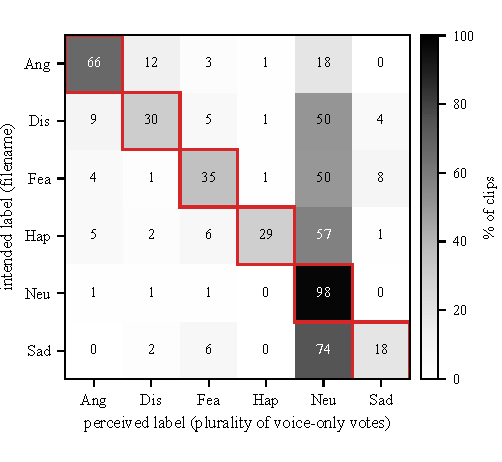
\includegraphics[width=0.98\linewidth]{../results/figures/fig1_confusion}
\vspace{-3mm}
\caption{Intended category (rows) against the plurality voice-only perceived
category (columns), row-normalised, over the \NUnamb{} clips with an unambiguous
plurality. The diagonal, which is what published CREMA-D accuracies are
scored against, carries less than half the mass.}
\label{fig:confusion}
\vspace{-5mm}
\end{figure}

Figure~\ref{fig:confusion} shows that the errors are not diffuse. Neutral is an
attractor: \NonNeutralAsNeutral\% of clips carrying a non-neutral instruction
are heard as neutral, and the perceived label is neutral for \NeutralShare\% of
the corpus against 14.6\% of the intended labels. Sad is the extreme case, with
\SadToNeutral\% of sad-intended clips heard as neutral against \SadRecovery\%
heard as sad. The natural reading is that acted sadness here is realised mostly
as lowered arousal, and lowered arousal in a short read sentence is hard for a
listener to separate from an unemotional one. Whatever the mechanism, a system
that labels every sad-intended clip \emph{neutral} is not making a mistake by
the listeners' standard; it is agreeing with them.

\subsection{A human ceiling}

How hard is each label to predict? For a human listener this can be answered
without any model. For each of the \NRatings{} voice-only judgements we removed
that rating, recomputed the plurality of the remaining raters for the clip, and
asked whether the held-out rater matched it. A listener agrees with the actor's
instruction \RaterVsIntended\% of the time and with their peers \RaterVsPeer\%
of the time. From the same audio, judged by the same people, the perceptual
target is eighteen points more predictable than the intended one.

It would be natural to conclude that the intended label is simply the noisier
target and that a recogniser trained on it is chasing information the recording
does not contain. Section~\ref{sec:results} shows that this conclusion is wrong,
and the way in which it is wrong is the more interesting half of the story.

\section{Experimental setup}
\label{sec:setup}

\textbf{Representations.} We use three, chosen to span capacity rather than to
be competitive. \textsc{mfcc}: 13 MFCC means and standard deviations (26-d).
\textsc{func}: a GeMAPS-style functional set~\cite{eyben2016gemaps} of 84
prosodic, spectral and cepstral descriptors, each summarised by eight
statistics---mean, standard deviation, median, interquartile range, the 1st and
99th percentiles and their range, and a linear slope over time---together with
voiced fraction, duration and jitter and shimmer proxies (677-d).
\textsc{ssl}: frozen WavLM Base+~\cite{chen2022wavlm} hidden states mean-pooled
over time and averaged over transformer layers 1--12 (768-d). The layer average
is fixed a priori so that no part of feature extraction is tuned against either
label set.

\textbf{Systems.} We pair those representations with logistic regression, a
Nystr\"om-approximated RBF classifier, histogram gradient boosting and a
two-layer MLP, giving \NSystemsWord{} systems in all. They are deliberately
ordinary. The aim is not to advance the state of the art on CREMA-D but to
obtain the kind of spread of systems a benchmark table contains.

\textbf{Training.} Every target is a distribution over the six categories, so
the three label regimes differ only in that distribution: one-hot on $y^{I}$,
one-hot on $y^{P}$, or the full $y^{S}$. All systems minimise cross-entropy
against it, which for a distributional target is obtained exactly by replicating
a clip once per category with that category's probability mass as its sample
weight. This keeps the comparison across regimes free of any confound from the
objective. Training is class-balanced by inverse frequency in every regime.
This is close to a no-op for $y^{I}$, whose classes are near-uniform by
construction (1{,}271 clips each, except neutral at 1{,}087), and it is
essential for $y^{P}$ and $y^{S}$, of which \NeutralShare\% is neutral:
unbalanced training against a neutral-dominated target simply collapses onto
neutral. Since the metric we report is deliberately prior-insensitive, so is the
training objective, and no regime is penalised for the shape of its label
distribution rather than its content.

\textbf{Protocol.} Speaker-independent five-fold cross-validation over the 91
actors; no actor appears in both a training and a test fold, and within each
training fold a further group of actors is held out for early stopping.
Hyperparameters were fixed once and shared across regimes. We report unweighted
average recall (UAR), the usual choice for class-imbalanced SER, and
additionally $R$, the probability that a system's output matches a randomly
drawn listener vote, which is the natural criterion when the reference is a
distribution. $R$ has a human reference: two listeners rating the same clip
agree \RaterRater\% of the time. Confidence intervals come from a clip-level
bootstrap with $2{,}000$ resamples, shared across systems so that paired
comparisons use common draws.

\section{Results}
\label{sec:results}

\begin{table*}[t]
\centering
\caption{Unweighted average recall (\%) under speaker-independent five-fold cross-validation over the 91 actors. Each block fixes the label a system was \emph{trained} on; within a block, UAR$_I$ and UAR$_P$ score the same predictions against the intended and the perceived label respectively, and $R$ is the probability that the prediction matches one randomly drawn listener vote. Best in each column in bold.}
\label{tab:main}
\small
\begin{tabular}{l@{\hspace{5mm}}ccc@{\hspace{5mm}}ccc@{\hspace{5mm}}ccc}
\hline
 & \multicolumn{3}{c}{trained on intended} & \multicolumn{3}{c}{trained on perceived} & \multicolumn{3}{c}{trained on soft} \\
\cline{2-4}\cline{5-7}\cline{8-10}
System & UAR$_I$ & UAR$_P$ & $R$ & UAR$_I$ & UAR$_P$ & $R$ & UAR$_I$ & UAR$_P$ & $R$ \\
\hline
FUNC-GB & 55.8 & 49.3 & 34.8 & 34.1 & 39.3 & \textbf{51.6} & 45.4 & 51.1 & 43.3 \\
FUNC-LR & 54.6 & 48.2 & 33.8 & 43.7 & 49.3 & 42.1 & 47.8 & 52.0 & 38.2 \\
FUNC-MLP & 54.6 & 48.1 & 34.6 & 45.5 & 50.6 & 40.6 & 49.1 & 52.5 & 36.9 \\
FUNC-RBF & 51.3 & 46.2 & 35.8 & 44.3 & 47.5 & 38.1 & 44.6 & 46.4 & 34.6 \\
MFCC-LR & 45.2 & 42.7 & 31.4 & 39.8 & 43.4 & 34.7 & 42.0 & 43.9 & 32.6 \\
MFCC-RBF & 48.1 & 44.1 & 33.6 & 42.1 & 44.9 & 35.3 & 42.1 & 43.5 & 32.6 \\
SSL-LR & \textbf{73.8} & \textbf{58.9} & 39.2 & 53.1 & \textbf{64.5} & 51.3 & 60.1 & \textbf{66.7} & \textbf{46.1} \\
SSL-MLP & 72.5 & 58.1 & \textbf{39.5} & \textbf{53.9} & 64.4 & 50.0 & \textbf{61.3} & 66.6 & 45.3 \\
\hline
\end{tabular}
\vspace{-4mm}
\end{table*}


\subsection{The numbers move}

Table~\ref{tab:main} gives every system under every regime. Under the standard
protocol---train on the filename label, score against it---our strongest system,
\TopSystem, reports \TopWAI\% accuracy, which is the range CREMA-D papers
usually occupy; the spread below it is a realistic one and not a set of straw
men. Scoring those identical predictions against the perceptual label instead
gives \TopWAP\%. Across the \NSystemsWord{} systems that substitution is worth
up to \SwingWAmax{} points of accuracy and \SwingUARmax{} points of UAR, with
nothing about the model changed.

Training on the perceptual labels moves things the other way. Averaged over
systems, fitting $y^{P}$ rather than $y^{I}$ buys \GainPerceived{} points of
UAR$_{P}$, and fitting the full vote distribution $y^{S}$ buys \GainSoft{}. That
the soft target beats the hard perceptual one is consistent with the soft-label
literature~\cite{ando2018soft}, and is the one place in this paper where we
reproduce a known result rather than report a new one. The perceptual regimes
also clear the human bar on $R$: the best perceptually trained entry matches a
randomly drawn listener \BestRPerceived\% of the time, where two listeners
rating the same clip agree only \RaterRater\% of the time. Predicting a listener
is easier than being one, which is what a model fitted to the vote distribution
is for.

None of this is surprising once stated---models fit the labels they are given
and are flattered by being measured against them---but it establishes the size
of the effect. Two papers reporting CREMA-D accuracy under the two conventions
are not describing the same quantity, and nothing in a typical experimental
section would reveal which convention was used.

\subsection{When the ranking moves}

\begin{figure}[t]
\centering
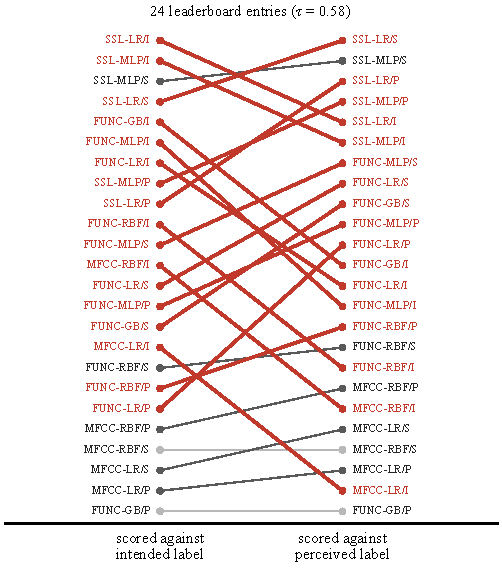
\includegraphics[width=0.98\linewidth]{../results/figures/fig2b_ranking_pooled}
\vspace{-3mm}
\caption{All \PoolEntries{} entries---every system under every training
label---ranked by UAR against the intended label (left) and against the
perceived label (right). Only the answer key differs. Entries that move three or
more places are drawn with heavier red lines.}
\label{fig:ranking}
\vspace{-5mm}
\end{figure}

Start with the narrowest version of the question. Fix the training label at
$y^{I}$, the standard protocol, and change only what the predictions are scored
against. Here the ordering essentially survives: Kendall's
$\tau = \TauIntended$, with \InvIntended{} of \NPairsIntended{} pairs changing
places, and the two systems in that pair separated by less than a tenth of a
point under either key. No inversion under any single training regime survives
the paired bootstrap. Architectures trained the same way remain comparable: the
two keys disagree about how good a system is, not about which is better.

A benchmark table is not in that position, and Figure~\ref{fig:ranking} shows
why. Such a table collects results from papers that made different and largely
undocumented choices about labels, so the unit that gets ranked is the entry,
not the architecture. Pooling our \PoolEntries{} entries, $\tau$ falls to
\PoolTau{} and \PoolInv{} of \PoolPairs{} pairs invert. The entry that wins
under intended labels (\PoolTopI) places \PoolWinnerDrop{} under perceived ones,
and the entry that wins under perceived labels (\PoolTopP) places fourth under
intended. Two groups reporting CREMA-D under different conventions would
disagree about which system is best, and each would be right about its own.

Were the two labels separated by a constant---were perceived labels simply
intended labels plus noise---every system would lose the same amount and the
ordering would be untouched. It is not, because the keys reward different
behaviour. A system that has learned the neutral attractor scores well against
perception and poorly against intent; a system that has learned to separate the
acted categories does the reverse. Model selection on CREMA-D therefore inherits
whichever choice of key was made, usually silently.

\subsection{What the two keys are asking for}

\begin{figure}[t]
\centering
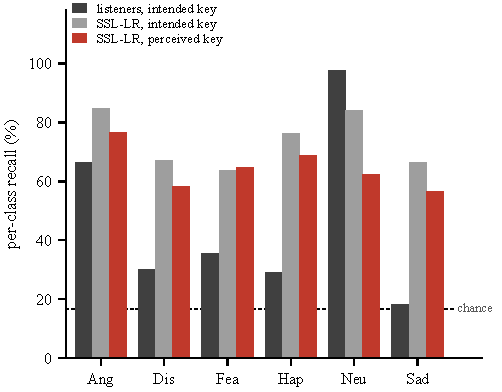
\includegraphics[width=0.98\linewidth]{../results/figures/fig3_per_emotion}
\vspace{-3mm}
\caption{Per-class recall for the strongest system under each key, against the
listeners' own recovery of the intended label. On the categories listeners find
hardest---sadness above all---the classifier reads the actor's instruction out
of the audio far better than they do.}
\label{fig:peremotion}
\vspace{-5mm}
\end{figure}

We do not claim the perceptual label is correct and the intended one wrong. They
set different tasks, and Figure~\ref{fig:peremotion} shows how differently.

Scored against intent, our strongest system recovers acted sadness for
\ModelSad\% of clips. Listeners manage \HumanSad\%. The same pattern holds for
disgust (\ModelDis\% against \HumanDis\%) and happiness (\ModelHap\% against
\HumanHap\%): on \NBeatHuman{} of the six categories a plain classifier reads
the actor's instruction out of the audio better than the listeners did, by as
much as \ModelBeatsBy{} points. It trails them only on neutral (\ModelNeu\%
against \HumanNeu\%), for the unremarkable reason that a class-balanced
classifier will not put half the corpus into one category. What it does not do
is find a different set of categories difficult: its per-class recall correlates
at $r = \CorrModelHuman$ with the listeners' across the six. The model finds the
same things hard, and is simply less troubled by them.

The acoustic trace of acted sadness, then, is present and consistent enough to
be learned. What listeners fail to do is not detect it but \emph{call it
sadness}: their criterion for the label demands more than these recordings
supply, and everything short of it collects in neutral. This reframes the choice
of key rather than settling it. Training against the filename label is not
fitting noise; it is training a system to recover the direction an actor was
given through a performance that listeners hear as unemotional. That is a
coherent objective and a classifier is good at it. It is not, however, the
objective that the phrase \emph{speech emotion recognition} is normally taken to
name, and a number obtained under it should not be read as a claim about what
anyone hears.

\section{Discussion}
\label{sec:discussion}

The narrow recommendation is that CREMA-D results should state which label set
they use, and that the perceptual labels---which require no new annotation, only
reading a file that ships with the corpus---should be reported alongside the
filename labels. Doing so costs nothing and makes results comparable.

The broader point concerns acted corpora generally. Such a corpus carries two
things at once: the instruction an actor was given, and the impression the
performance leaves. Both turn out to be recoverable from the audio, which is
what makes the choice between them a real one rather than a choice between
signal and noise. A corpus that ships perceptual ratings makes that choice
explicit; CREMA-D ships them, and the community has settled by default on the
key that puts the reference label out of reach of the listeners the system is
nominally imitating.

\textbf{Limitations.} The perceptual labels are themselves a consensus over
roughly nine raters, with the reliability reported in
Section~\ref{sec:gap-rec}; a plurality over nine crowd workers is a noisy
estimate of a distribution, and clips near a tie are close to arbitrary. Our
systems are conventional and CPU-scale, so the reordering is demonstrated on the
kind of spread found in benchmark tables rather than among frontier models;
whether it also occurs among a set of near-identical large models is open.
Finally, everything here concerns one corpus. CREMA-D is the convenient case
because it distributes both labels for the same clips, but the question it
raises---which reading of an acted corpus is being scored---applies wherever
directed emotion is used as ground truth.

\vfill\pagebreak

\section*{Compliance with ethical standards}

This is a secondary analysis of CREMA-D~\cite{cao2014cremad}, a corpus released
publicly by its authors under the Open Database License. No new recordings and
no new human ratings were collected for this work, and no identifying
information about the actors or the raters is used beyond the demographic fields
already distributed with the corpus.

\bibliographystyle{IEEEbib}
\bibliography{refs}

\end{document}
